\documentclass{beamer} 

%%%%%%%%%%%%%%%%%%%%%%%%%%%%%%%%
% PACKAGES
% Stuff we import to make LaTeX do more.

% Gives us block comments.
\usepackage{comment}

%%%%%%%%%%%%%%%%%%%%%%%%%%%%%%%%
% THEME METADATA
% Playing with themes... what others are there?
\usetheme{Warsaw}
%\usetheme{Berlin}

% Themes can have colors as well...
% Again, what is available?
\usecolortheme{seahorse}
\usefonttheme[onlylarge]{structuresmallcapsserif}

%%%%%%%%%%%%%%%%%%%%%%%%%%%%%%%%
% PRESENTATION METADATA
\title{A Walk in the Commons} 
\author{Mel Chua, Matt Jadud} 
\date{December 2, 2011} 

\begin{document}

% Generates the title of the talk.
\titlepage

\begin{frame} 
\frametitle{outline}
\tableofcontents
\end{frame} 

\section{Open Communities}
\begin{comment}
* What is open / what are open communities?
** What's open source/content?
** some projects you may have heard of (Firefox, Wikipedia, etc)
** some you may not have (Wikiotics, CivX, FreeCiv, Civicommons, Sahana, CiviCRM)
** it's not just Linux - a lot of this stuff runs on other platforms too (Windows, Mac, web-based) "no, we are not trying to get you to reinstall your computer" (but if you're interested, we're happy to help)
** the Four Freedoms (made for software)
*** Freedom / friends / ?
** creative commons (made for content)
** it's more than licensing... what's "the open source way," some characteristics of those communities (realtime transparency, etc)
\end{comment}

% I'm going to use a line of comment markers to indicate that there is a new
% frame happening. It will make things a bit a bit easier to read.

%%%%%%%%%%%%%%%%%%%%%%%%%%%
\begin{frame} 
\frametitle{what are open communities?}

\huge
\begin{center}
\begin{minipage}{7cm}
A distributed group of \alert{volunteers} committed to \alert{giving away} their efforts.
\end{minipage}
\end{center}

\end{frame} 

%%%%%%%%%%%%%%%%%%%%%%%%%%%
\begin{frame} 

% 'T' aligns the top of the columns, 'c' the center.
\begin{columns}[T] 
% ** some you may not have (Wikiotics, CivX, FreeCiv, Civicommons, Sahana, CiviCRM)
\column{1.5in} 
\begin{itemize}
	\item Firefox
  \item Wikipedia
	\item Wikiotics
	\item CivX
	\item FreeCiv
	\item Sahana
\end{itemize}

\column{1.5in} 
% Framebox puts a frame around the image... not what I want here.
%\framebox{
\includegraphics[height=2cm]{images/ff-logo.png}}

\includegraphics[height=2cm]{images/ff-logo.png}
\vspace{1cm}

\includegraphics[height=2cm]{images/wiki-logo.png}
\vspace{1cm}
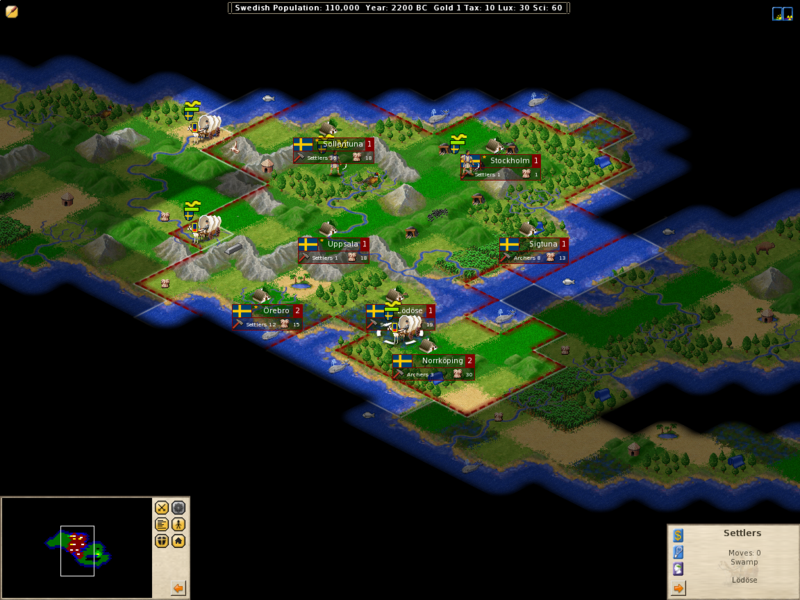
\includegraphics[height=2cm]{images/freeciv-logo.png}

\end{columns}
\end{frame} 


\section{Opportunities for Learners}
\begin{comment}
* What can your students do?
** One example (pick one - Fedora & your first-year class)
** Documentation
** Translation
** Gardening
** Bug fixing
** Testing
** Artwork/design
** Marketing/outreach
** Being active and vocal users (use open source in outreach/service projects - for instance, Mo & the Girl Scouts) / advocacy
** Legal/licensing work (very, *very* basic stuff)
** it's the non-programming skills that are usually in most need by these communities, because nobody knows about them / how to do them, so you can almost become domain "experts" in a project
** Creative repurposing - bringing a project into a new domain it wasn't necessarily originally designed for
\end{comment}

\begin{frame} 
\frametitle{what can (your) students do?}
\end{frame} 


\section{Opportunities for Researchers}
\begin{comment}
Researchers: they exist! (10 seconds each, no more.)
* coleman - ethics in foss communities
* krafft - innovation diffusion
* benkler - "law stuff"
* von hippel - economics
* lawler - wikiversity formation
* dennys and martin - semantic mediawiki
* davis and jabeen - legitimate peripheral participation
* government adoption paper whose author name I forgot
* Mini Case Study: CC licensed video in Zach's research
\end{comment}

\section{Opportunities for Educators}
\begin{comment}
* What can you do?
**  Who's there to help you?
** Who's working on this?
\end{comment}

\section{Value Proposition}
\begin{comment}
* Why make the connection?
** Legitimate Peripheral Participation & situated learning
*** Students can engage -- the currency is desire and energy
** Community of educators
*** Local (institutional)
*** Global (distributed)
*** A community of practice as opposed to a research community
\end{comment}

\section{Cases}
\begin{comment}
* Cases
** Case study: Scientific Computing (we know this target exists)
*** Target user: a senior physics major who knows some C, and wants to either 1) contribute to a project or 2) do some research and feed it back into a community
*** Write wiki articles instead of writing a paper.
*** http://www.scipy.org/Getting_Started
*** http://www.opensourcephysics.org/
**** Extend with projects that run on the EC2 compute cloud / GPGPUs
*** Automation of experiments / Arduino
\end{comment}

\section{Paths Well Traveled}
\begin{comment}
* existing programmes and opportunities
** GSOC
** Creative Commons uni program
** Wikipedia Prof Program
** TOS (sorta) / POSSE? (maybe)
\end{comment}

\section{Challenges}
\begin{comment}
* Challenges of doing open community stuff with students
** Some problems remaining to solve (for instance, IRC's interface sucks, community members don't always understand the "shoot self in foot" redirection need, hard to find projects, etc)
\end{comment}

\end{document}
